% !TEX root = main.tex

\section{Introduction}
\label{sec:intro}

The ability to grasp objects lies at the heart of robotic manipulation and therefore is fundamental to enabling robots to have complex physical interactions with their environment. 
Grasping a variety of unknown objects is challenging due to sensor and actuator uncertainty and uncertainty with respect to an object's shape, mass distribution, texture properties, etc. 
Recently, deep neural networks have been used, with significant success, to address these challenges. 

Within the context of this paper, we will make three assumptions. 
First, we will be grasping objects from a flat, clutter-free surface, such as an uncrowded table top. 
Second, we assume we have a method of generating \textit{grasp candidates}. 
Last, the robot has either an on-board camera or the environment the robot is operating in has a camera. 
Given an image of the scene captured by the camera, our goal is to evaluate which of these candidate grasps are likely to succeed. 
This creates a binary classification task, where the labels are grasp success and grasp failure. 

During execution, we can imagine that our robot with sample several grasps, execute a grasp that has been predicted to be successful via our classification method.  

For our data set we will use the Dexerity Network (DexNet) 2.0 data set, presented in~\cite{mahler2017dex}. 
The data set has 6.7 million grasps definitions, images and analytical grasp metrics, that we further detailed in \sref{sec:data_set}. 
The authors of the data set trained a Grasp Quality Convolutional Neural Network (GQ-CNN), which achieved 85.7\% accuracy on their classification task.

\rhnote{explicitly list contributions}

We first review related work (\sref{sec:related_work}) and further detail the data set (\sref{sec:data_set}). 
Given our data set, we formally define our problem statement (\sref{sec:problem}) and then explore various data sets using the pre-trained GQ-CNN (\sref{sec:balance}). 
We explore other architectures (\sref{sec:archs}) and conclude with a brief discussion (\sref{sec:discussion}). 

\begin{figure}[t!]
    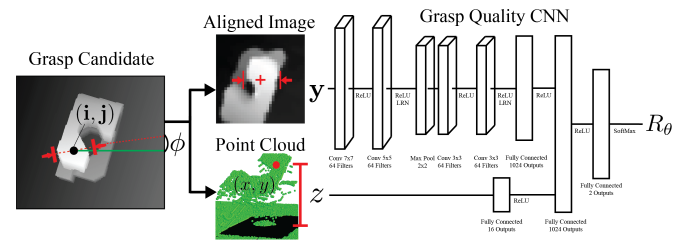
\includegraphics[width=0.99\columnwidth]{figs/dexnet.PNG}
\caption{Fill in caption. From \cite{mahler2017dex}} \label{fig:dexnet_network}
\end{figure}

\begin{comment}

To accomplish the same task, we will be experimenting with new architectures, intput formats, other modifications described in~\sref{sec:questions}.
Most of the recent machine learning papers in robotics present a problem, dataset and, usually, an optimized convolutional neural network with some architecture and input format. 
Our goal is to explore the process of finding that CNN and exploring the factors that effect performance. 
While our results will only be verified according to this data set, and therefore cannot be generalized to all CNNs, we hope to gain intution, understanding, and, hopefully, a higher accuracy. 
Having explored various components, we will optimize our final, best architecture. 
\end{comment}
